\section{Path Planning}

In the domain of robotics, there are hundreds if not thousands of different path planning implementations some of which present totally new formulations for planning but most present incremental improvements that decrease the computational resources, or optimize some custom metric. The goal of this paper is to present a handful of the most popular (and historically important) path planners that have made a significant impact in robotics and have become defacto standard benchmarks against which all other planning algorithms compare their performance. 

This paper will cover A*, RRT, PRM, and Dijkstra's Shortest Path. Each of these algorithms is graph-based in so much as they utilize a graph or tree as the data structure from which the algorithm will attempt to generate the shortest path. While algorithms like A* and Dijkstra typically can be given a preexisting graph to traverse, algorithms like RRT and PRM implement a type of Monte Carlo random sampling to generate the graph/tree that they traverse, later after the path generation phase of the planner. This section will cover each of the aforementioned algorithms in broad strokes, describing the general construction and planning mechanism(s) at play.

\subsection{Global vs Local Planners}

Before diving into the details of each planner, it is important to clear up the role of these planners and how this role effects the type of planning being performed in the system. Planners can generally be categorized as either \textbf{global} and \textbf{local}.  

A global planner provides an idealized "global" path between the starting location and the target destination. Typically this plan is optimizing some metric(s) such as shortest distance, curvature constraints, and/or static object avoidance. In a perfect world, an autonomous robot/vehicle would only require a global planner and a means of localizing itself (from sensor measurements); however, dynamic/uncertain obstacles coupled with imperfect sensing, mapping, and localization require robots to be more robust to uncertainty. The planning algorithms shown in the paper are all examples of global planners, as we have already made the assumption that the environment is static. 

To combat environmental uncertainty, roboticists developed the idea of local planners. Functionally, local planners use onboard sensor measurements to account for uncertainties in the global path in realtime. This is accomplished by planning deviations from the global path to maintain feasibility and to remain unobstructed. Additionally, local planners can include computation to smooth the global path and provide waypoints to the control system. However, these planners are more than just post-processing of the global path in so much as they need to be aware of the pose, dynamics, kinematics, constraints, and sensor inputs of the robot/vehicle.

\subsection{Path vs Motion Planning}
Frequently, the terminology of path planning is conflated with that of motion planning. While related, these concepts are very different and each solves a different problem. In path planning, the objective is to find the path through an environment that optimizes some metric and obeys specified constraints. Typically this metric is distance or cost and the constraint is to maintain a feasible and obstacle free path between the starting and ending points. 

Motion planning, on the other hand, uses path planning as an input to determine how the path should be traversed through time. This means not only planning the position of the path (e.g path planning) but also planning the velocity, acceleration, and often the jerk of a robot as it follows the given path. Almost always, motion planning requires the ability to compute derivatives of the path position. 

\subsection{Planning Algorithms}

The first category of planning algorithms are so-called \textbf{Graph-Search}. The primary mechanism these planners employ is to construct a graph from a map. Once this has been achieved, different algorithms, heuristics, and operations can be applied over the graph to endeavor to find the shortest path between two nodes that exist in that graph. Occupancy grid maps are ideal for the such path planners in that it is trivial to translate the grid map into a graph data structure by assuming that every pixel in the grid map is node in the graph, and then formulate the connectivity rules as desired (see \textbf{connected-4} or \textbf{connected-8} above). 

\subsubsection{Dijstra's Shortest Path}
The predecessor of almost all graph-search planners is Dijkstra's shortest path. This algorithm was invented by Dutch mathematician Edsger Dijkstra in Norway in 1956 \cite{dijkstra1959note}. It implements a type of breadth-first search that will traverse an undirected graph, until it has found the shortest route between two nodes within the graph. 

The implementation found in this paper for Dijkstra's algorithm uses an occupancy grid map to generate a dense graph. Cells in the map that have an occupancy value over a certain threshold are assumed to be occupied. The algorithm works by computing the cost of the current node, and then determining the total cost of each neighbor from the current node. The neighbor with the least cost is expanded in the same way until either the entire graph has been explored or the path from the start and end nodes has been determined. See algorithm for more details.

\label{Dijkstra}
\begin{algorithm}
  \caption{Dijkstra's Shortest Path}
  \begin{algorithmic}[h!]
  % \renewcommand{\algorithmicrequire}{\textbf{Input: Graph, startNode, targetNode}}
  % \renewcommand{\algorithmicensure}{\textbf{Output: Path}}
   \FOR { node in Graph }
   \STATE $\text{node.score} := \infty$
   \STATE $\text{node.visted} := \text{false}$
   \ENDFOR

   \\ \textit{Solve Graph} :
   \STATE $\text{starNode.score} := 0$
   \WHILE { ( true ) }
  \STATE $\text{currentNode} := \text{nodeWithLowestScore(Graph)}$
  \STATE $\text{currentNode.visted} := \text{true}$

    \FOR { ( node in currentNode.neighbors ) }
    \IF{ ( $\text{node.visited} == \text{false}$ ) }
    \STATE $\text{newScore} := \text{calculateScore(currentNode, node)}$
    \IF{ ( $\text{newScore} < \text{node.score}$ ) }
    \STATE  $\text{node.score} := \text{newScore}$
    \STATE  $\text{node.routeToNode} := \text{currentNode}$
    \ENDIF
    \ENDIF
    \ENDFOR
    \\
    \\ \textit{Return Path} :
    \IF{ ( currentNode == targetNode ) }
    \RETURN build{Path(targetNode)}
    \ENDIF

    \\
    \\ \textit{Raise Error if No Path is Found} :

    \IF{nodeWithLowestScore(graph).score == $\infty$}
    \RETURN ERROR: No Path Found
    \ENDIF

   \ENDWHILE

  \end{algorithmic} 
  \end{algorithm}

While this algorithm is simple and guaranteed to find the shortest path in the graph, assuming it exists, it cannot predict the efficiency of how well it is at finding the shortest path. This is predominately attributable to the fact that the algorithm is a generalization of a breadth-first search, blindly expanding every node closest to it without any concern to focus the direction of the search towards more likely paths (e.g. in the direction of the goal state).

% 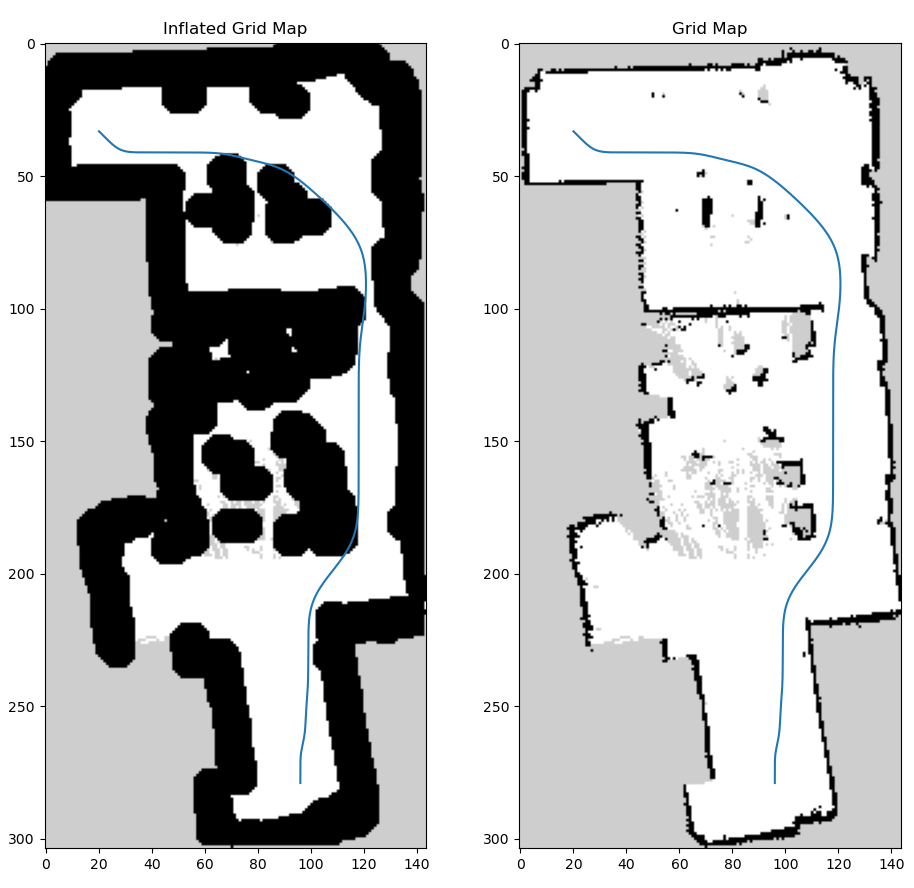
\includegraphics[scale=.3]{dijkstra.png}

% \subsection{Dijkstra Shortest Path}




\begin{figure}[h]
    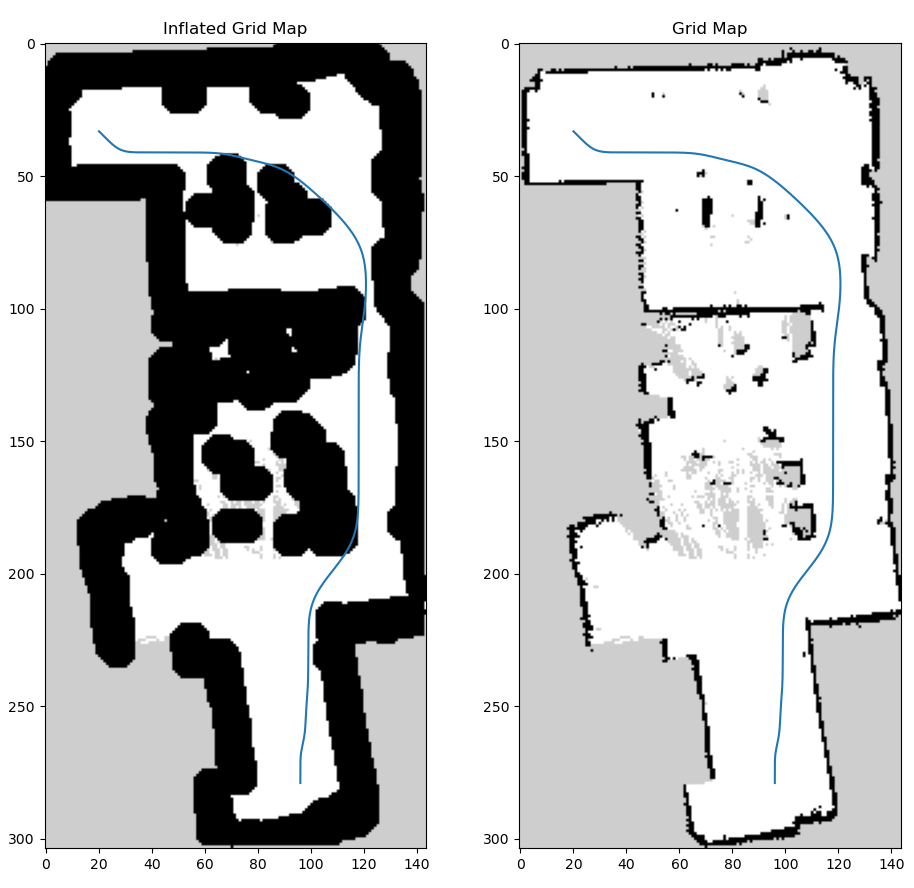
\includegraphics[width=8cm]{dijkstra}
    \centering
    \label{fig:Dijkstra}
    \caption{Dijkstra Algorithm in SLAM generate Map}
\end{figure}


\subsubsection{A*}

The A* algorithm was developed at the Stanford Research Institute in 1968, for the historically significant robot Shakey, being used in some of the earliest pioneering research into mobile robotics \cite{Hart1968}. It is both the literal and conceptual successor to Dijkstra's algorithm. Both implement a graph-search; however, the primary improvement of A* is the addition of a search heuristic that improves the ability of the algorithm to focus on expanding nodes in the direction of the goal state.  

Unlike Dijkstra's algorithm, the addition of a heuristic provides the planner with the ability to preferentially search in a given direction and will traverse nodes that are more likely to be approaching the goal node fom the starting node. So long as the heuristic is quick to compute and admissible (an exact or under estimate of the actual distance to the goal node), we can use a search heuristic to drastically improve the planners convergence rate.

A* is extremely similar to Dijkstra's algorithm described above. The key difference is how A* computes the cost of getting to the current node, and then computes the cost of traversing to each neighboring node plus the addition of a heuristic cost from each neighbor to the goal state. The inclusion of a heuristic cost allows A* to preferentially choose to visit neighbors that are closer to the goal state by choosing the neighbor with the lowest combined current plus heuristic cost. See algorithm for more details.

\label{A*}
\begin{algorithm}
  \caption{A* Heuristic Search}
  \begin{algorithmic}[1]
   \FOR { ( $\text{node in Graph}$ ) }
    \STATE $\text{node.gScore} := \infty$
    \STATE $\text{node.fScore} := \infty$
    \STATE $\text{node.visted} := \text{false}$
   \ENDFOR

   \textit{Solve Graph} :
   \STATE $\text{starNode.gScore} := 0$
   \STATE $\text{starNode.fScore} := 0$
   \WHILE { ( true ) }
  \STATE $\text{currentNode} := \text{nodeWithLowestScore(Graph)}$
  \STATE $\text{currentNode.visted} := \text{true}$

    \FOR { ( node in currentNode.neighbors ) }
    \IF{ ( $\text{node.visited} == \text{false}$ ) }
    \STATE $\text{newScore} := \text{calcScore(currentNode, node)}$
    \IF{ ( $\text{newScore} < \text{node.g}$ ) }
    \STATE  $\text{node.gScore} := \text{newScore}$
    \STATE  $\text{node.fScore} := \text{newScore} + \text{calcHeuristic(nextNode, targetNode)}$
    \STATE  $\text{node.routeToNode} := \text{currentNode}$
    \ENDIF
    \ENDIF
    \ENDFOR
    
    \\ \textit{Return Path} :
    \IF{ ( currentNode == targetNode ) }
    \RETURN build{Path(targetNode)}
    \ENDIF

    
    \\ \textit{Raise Error if No Path is Found} :

    \IF{nodeWithLowestScore(graph).score == $\infty$}
    \RETURN ERROR: No Path Found
    \ENDIF

   \ENDWHILE

  \end{algorithmic} 
  \end{algorithm}

A* has made a tremendous impact on the world of robotics and today is the defacto standard for simple path planning tasks. Unfortunately, both A* and Dijkstra suffer from the necessity to generate a graph of the environment. As previously mentioned, this usually involves the conversion of a grid map into graph. While not always an issue, the dimension of the grid map corresponds to the need to generate a larger search graph, which requires either algorithm to spend more time to compute the shortest path. Unlike Dijkstra's, the heuristic driven nature of A* also means that it is typically far more efficient of a search than Dijkstra's algorithm over the same search graph. 

% 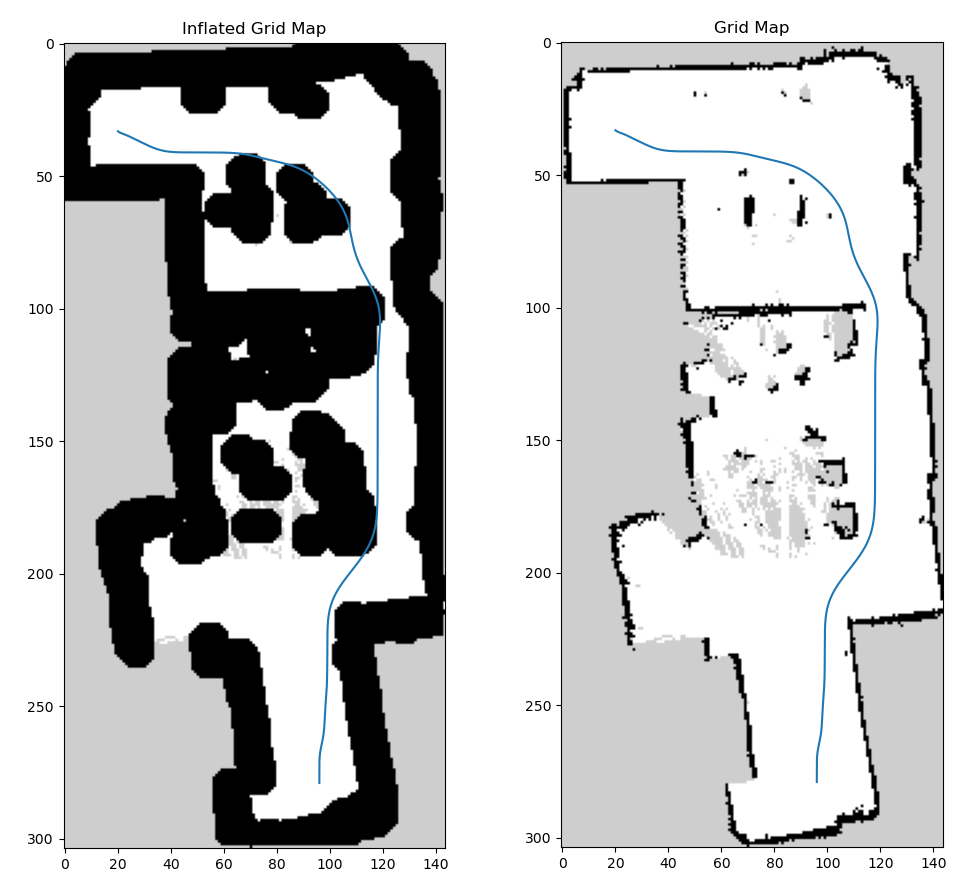
\includegraphics[scale=.3]{astar.png}

\begin{figure}[h]
    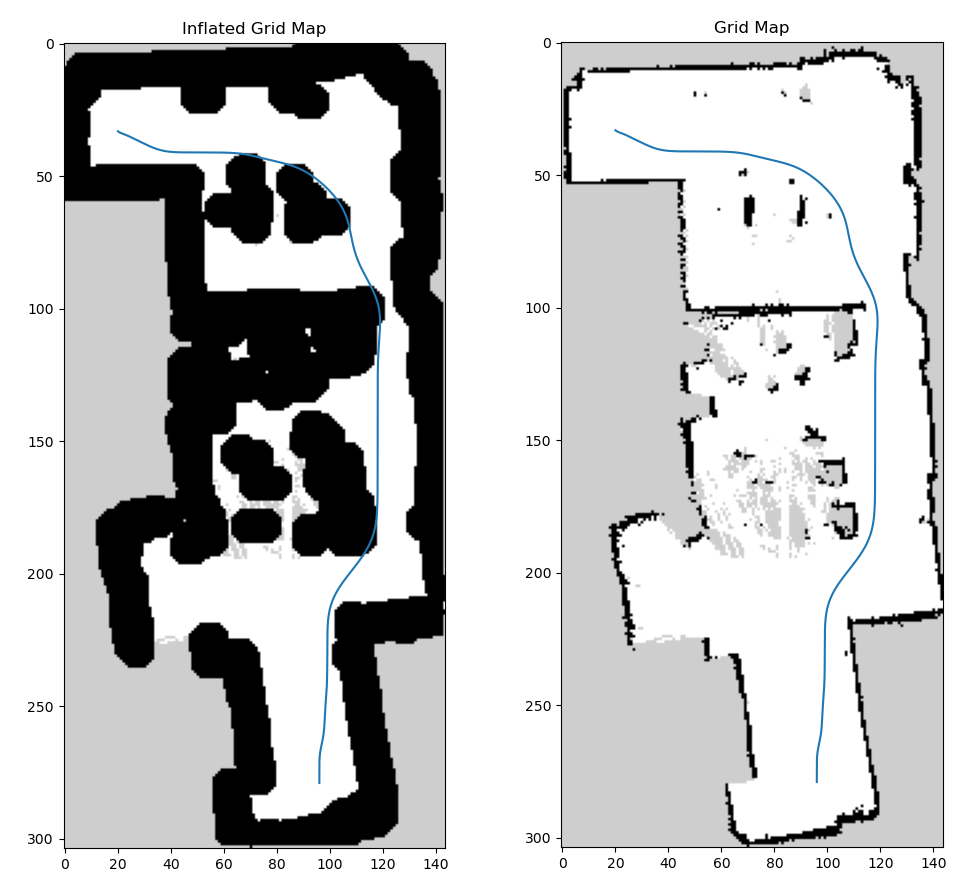
\includegraphics[width=8cm]{astar}
    \centering
    \label{fig:Astar}
    \caption{A Star}
  \end{figure}

\subsubsection{Probabilistic Road Maps}

While graph-search planners have been popular and practical historically, methods like Dijkstra's and A* can only be as efficient as the size, resolution, and connectivity of their graph permits. Depending on how these graphs were generated, they often suffer from the inability to efficiently scale as the size of a given map increases, leading to unacceptable latency and computation times, known as the curse of dimensionality.

To address the problem of high graph densities, the algorithm Probabilistic Road Maps (PRM) was developed. PRM has two main stages; graph creation via random sampling, and path computation by directly applying Dijkstra's algorithm. The broad objective of PRM is to decrease the density of the search-graph by applying uniform sampling as the mechanism for generating graph nodes within the map \cite{PRM}. The compromise this method makes is the reduction of graph generation and graph traversal times in exchange for a lower fidelity map that is no longer pixel accurate to the map.

PRM works by randomly selecting a number of points within the domain of the map. It will first check whether or not the randomly selected point is an obstacle. If the sample is contained within an obstacle, the algorithm will redraw random samples until it finds a point that is \textit{free}. This point is then added to an ever growing graph, so long as the edge connecting this new node and the previous nodes in the graph do not intersect obstacles. Once this has been performed for a sufficient number of random samples, the graph or 'roadmap' now exists. The second phase of the algorithm merely selects a starting and target nodes, in the graph and applies a graph-search algorithm between those two endpoints.

This technique is not only faster for the graph generation portion of the algorithm, but since the graph it generates is typically over an order of magnitude less dense than an equivalent grid map based graph, finding the shortest path between two points on this "sampled" graph results in significantly faster graph traversal. It should be noted that unlike the other methods, PRM is only optimal within the limit as the number of samples becomes infinite. This means that unlike A* traversing a dense grid-based graph, PRM with a finite sample size is unlikely to find the optimally shortest path; however it does provide a locally optimal path across its sampled-graph. This behavior demonstrates how PRM needs to be tuned to its targeted application for effective results.  

\label{Probalistic Road Maps}
\begin{algorithm}
  \caption{Roadmap Construction}
  \begin{algorithmic}[1]

  \renewcommand{\algorithmicrequire}{\textbf{Input:} }
  \renewcommand{\algorithmicensure}{\textbf{Output:} }
  \REQUIRE 
    \text{    n: number of nodes in roadmap} \linebreak
    \text{    k: number of closest neighbors to examine for each configuration} \linebreak

  % \textbf{Output:} \linebreak
  \ENSURE  \linebreak
    \text{    A roadmap G = (V, E)} \linebreak

  \hrulefill 

  \STATE \text{$V \leftarrow \emptyset$}
  \STATE \text{$E \leftarrow \emptyset$}

   \WHILE { $\lvert V \rvert < n$ }

    \STATE \textbf{repeat}
    \STATE $\text{     q} \leftarrow \text{random sample from Configuration Space } \mathcal{Q}$
    \STATE \textbf{until} \text{q is collision-free}
    \STATE $V \leftarrow V \cup \text{\{q\}}$
   \ENDWHILE
   \FOR {  $\textbf{all } \text{q} \in \text{V}$  }
   \STATE $N_q \leftarrow \text{the k nearest neighbors of q from V by \textit{dist}}$
    \FOR { $\textbf{all } q^{\prime} \in N_q$  }
    \IF { ($\text{q, } q^{\prime}) \notin \text{E \textbf{and }} \Delta(\text{q, } q^{\prime}) \ne 0$ }
    \STATE $\text{E} \leftarrow \text{E } \cup \{ ($\text{q, } q^{\prime}) \}$
    \ENDIF
    \ENDFOR

   \ENDFOR

  \end{algorithmic} 
  \end{algorithm}

% 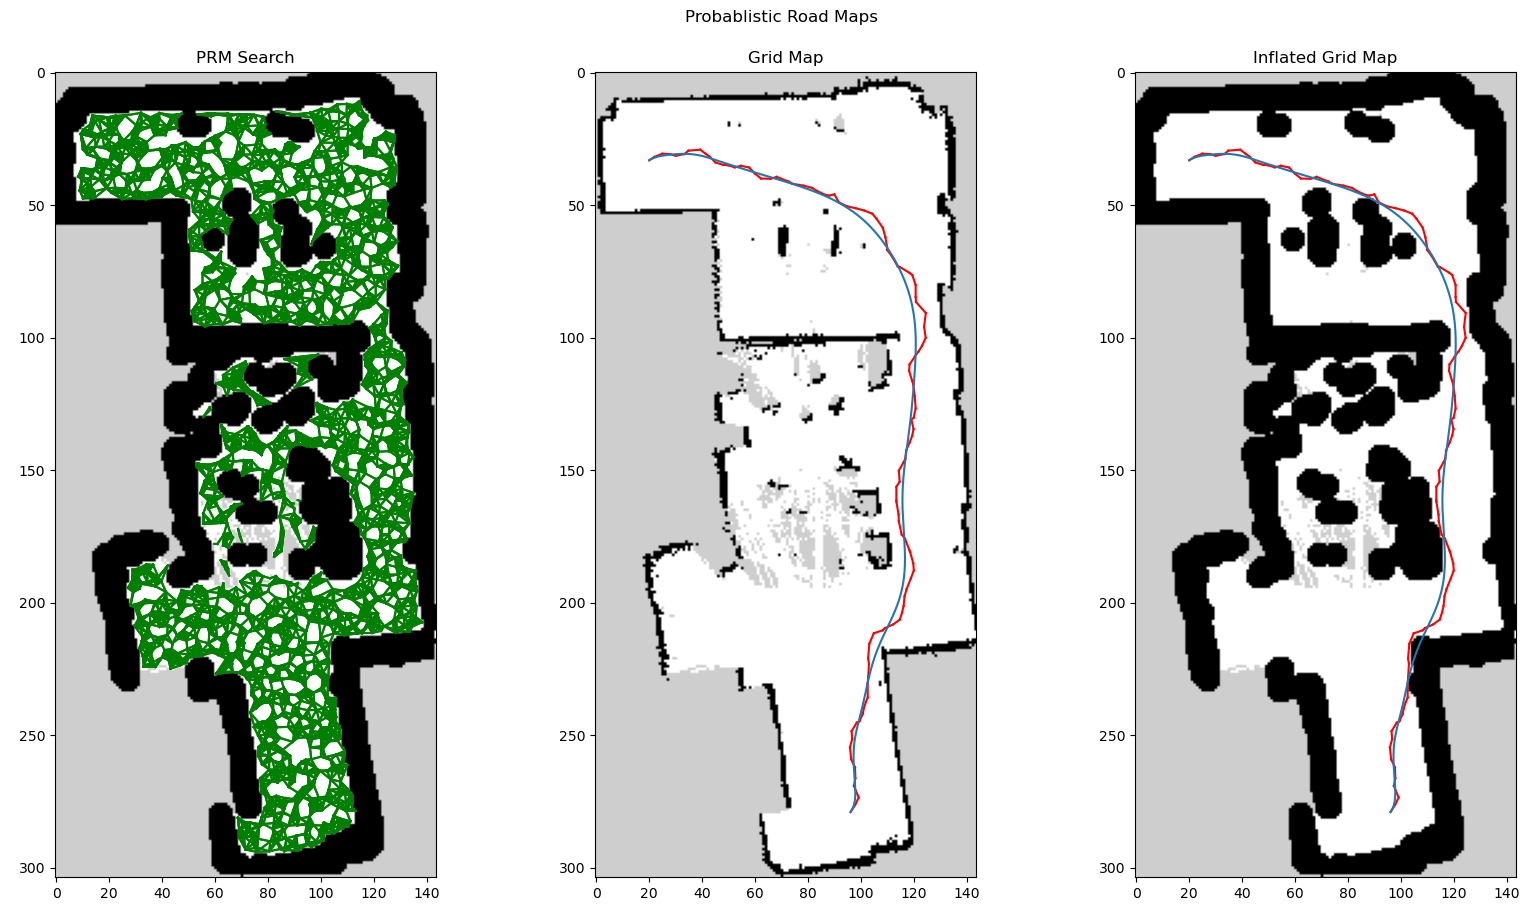
\includegraphics[scale=.23]{probablistic_road_map.png}
\begin{figure}[h!]
    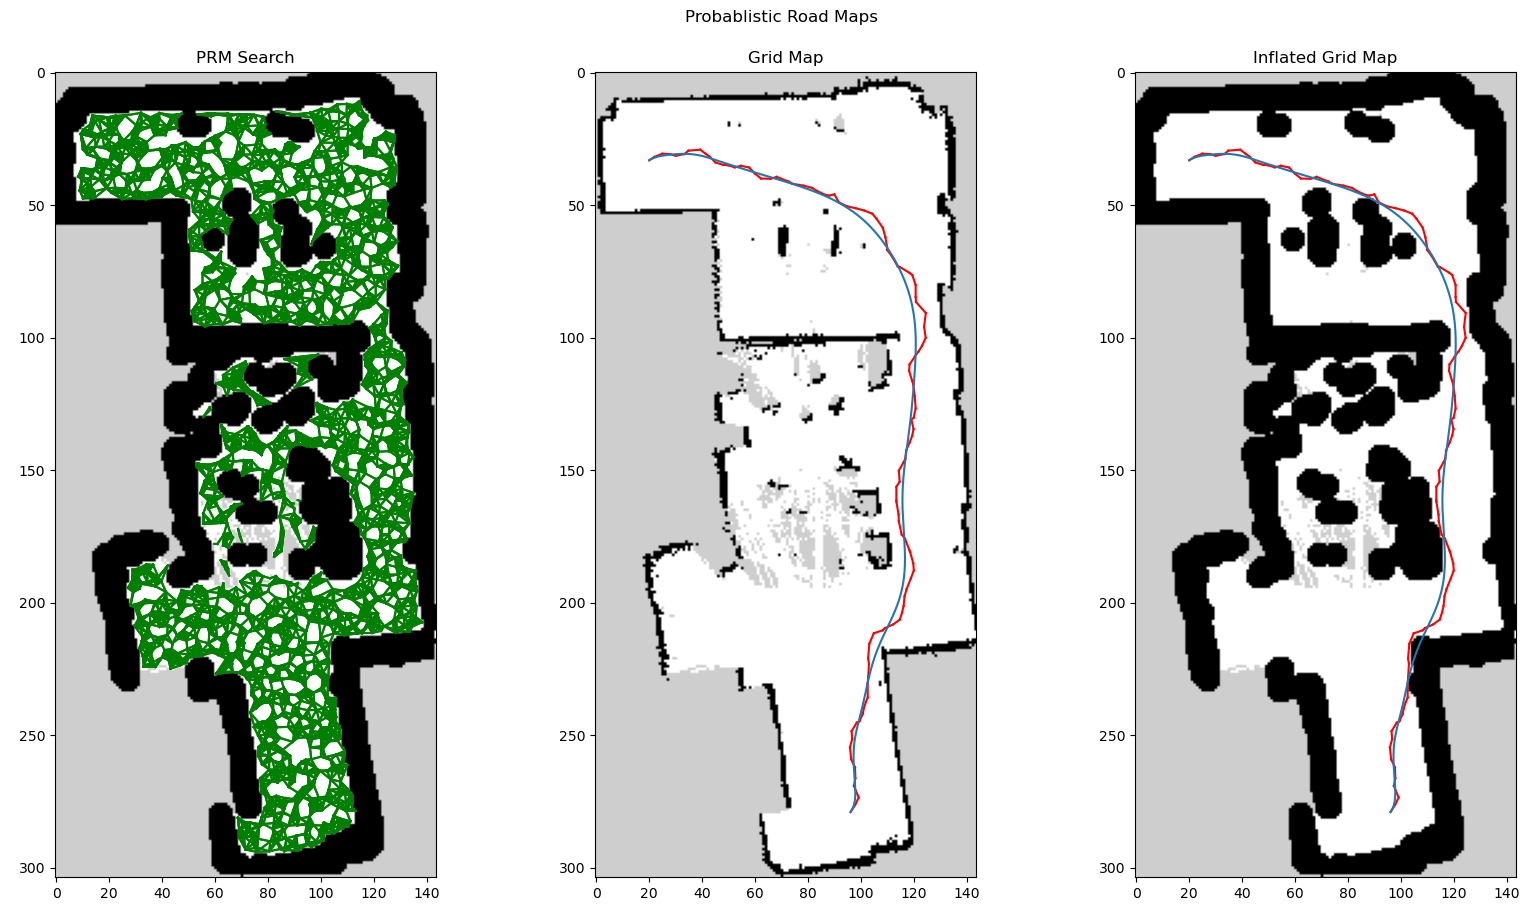
\includegraphics[width=8cm]{probablistic_road_map}
    \centering
    \label{fig:PRM}
    \caption{Probabilistic Road Maps}
  \end{figure}

\subsubsection{Rapidly Exploring Random Trees}

Similar to PRM, Rapidly Exploring Random Trees (RRT), also attempts to leverage random sampling to improve the sample efficiently and reduce the graph generation time \cite{LaValle1998RapidlyexploringRT}. The primary difference between PRM and RRT is their data structures and how additional nodes are inserted into this data structure. While PRM utilizes a graph, the RRT class of algorithms use a tree structure. Tree structures possess several benefits but also impose several constraints on the representation of the map that these algorithms generate. 

The most useful aspect of using a tree is the simplicity in determining the final path. Unlike all of the graph-based methods that require iteratively searching over a large portion of nodes in the graph to determine the shortest path, a tree structure is a very simple structure that lends itself to recursive solutions. Since unlike a node in a graph, a node in a tree can only possess one predecessor, one need only begin at the final target node and recursively make a list of each predecessor node, until the starting node is reached.

Like PRM, RRT will randomly sample its map, check that these random points are not obstacles in the map (resample if true) and then create a tree by tieing that random point into the nearest node of the tree, by taking a step of size $\DeltaS$ towards the random point, from its closest node on tree. At this new location, it will create a new node that is parented to the nearest neighbor previously mentioned. 


% Similar to PRM, RRT is not guaranteed to find the shortest path between two nodes even in the limit as the number of samples trends towards infinitely sample the map. Unlike PRThis is due to the static nature of the tree generation. 

\label{RRT}
\begin{algorithm}
  \caption{RRT Construction}
  \begin{algorithmic}[1]

  \renewcommand{\algorithmicrequire}{\textbf{Input:} }
  \renewcommand{\algorithmicensure}{\textbf{Output:} }
  \REQUIRE 
    \text{    $q_0$:the configuration where the tree is rooted} \linebreak
    \text{    n: the number of attempts to expand the tree } \linebreak

  \ENSURE  \linebreak
    \text{    A tree T = (V, E) that is rooted at $q_0$ and has $\le $ n configurations } \linebreak

  \hrulefill 

  \STATE \text{$V \leftarrow \{q_0\}$}
  \STATE \text{$E \leftarrow \emptyset$}

  \FOR {  i = 1 to n  }
  \STATE $q_{rand} \leftarrow$ a randomly chosen free configuration
  \STATE $q_{near} \leftarrow$ closest neighbor of q in T
  \STATE $q_{new} \leftarrow$ node a dist $\Delta S$ from $q_{near}$ to $q_{rand}$
    \IF { $q_{new}$ is collision-free }
      \STATE V $\leftarrow$ V $\cup$ \{$q_{new}$\}
      \STATE E $\leftarrow$ E $\cup$ \{($q_{near}$, $q_{new}$ )\}
      \RETURN $q_{new}$
    \ENDIF
    \RETURN 0
  \ENDFOR

  \end{algorithmic} 
  \end{algorithm}